\begin{frame}
  \begin{block}{Custos utilizados no experimento}
    \begin{figure}
      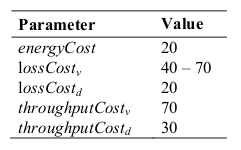
\includegraphics[scale=0.47]{./Figures/costsTable}
    \end{figure}
  \end{block}
  \begin{block}{Função custo}
    \begin{figure}
      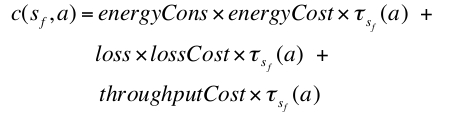
\includegraphics[scale=0.37]{./Figures/form4}
    \end{figure}
  \end{block}
  Custos não possuem dimensões. São utilizados para indicar o peso de cada
  parâmetro na função
\end{frame}

\begin{frame}{Análise da política ótima}
  \textit{Voice loss cost}
  \begin{block}{$ \text{lossCost}_v = 40$}
    \begin{itemize}
      \item Todas as requisições são atendidas pela \textit{femtocell}, até o
      seu limite de usuários
    \end{itemize}
  \end{block}
  \begin{block}{$40 < \text{lossCost}_v < 70$}
    \begin{itemize}
      \item Escolha da célula influenciada pelo grau de congestionamento da
      \textit{femtocell}
      \begin{itemize}
        \item $CR_f$ baixo: \textit{femtocell}
        \item $CR_f$ alto: \textit{macrocell}
      \end{itemize}
    \end{itemize}
  \end{block}
  \begin{block}{$\text{lossCost}_v = 70$}
    \begin{itemize}
      \item Voz e dados devem utilizar a \textit{macrocell}, a menos que esta
      esteja congestionada
    \end{itemize}
  \end{block}
\end{frame}

%\begin{frame}
%  Aumento do custo de perda, diminui importância do custo de consumo de energia
%  \begin{figure}[h]
%  	\begin{center}
%      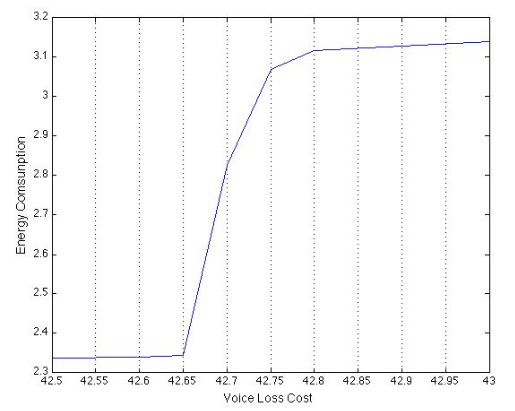
\includegraphics [scale=0.4]{./Figures/powerVSloss}
%      \caption {Consumo médio de bateria X custo de perdas de voz
%      \cite{green-markov}.}
%  		%\label{fig:arq-imuno}
%  	\end{center}
%  \end{figure}
%\end{frame}

\begin{frame}
  Aumento do custo de perda, diminui importância do custo de consumo de energia
	\begin{figure}[!htb]
		\centering
		\subfloat[Consumo vs $\textit{lossCost}_v$]{
			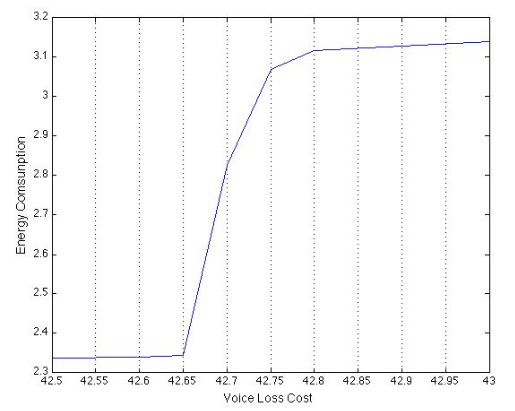
\includegraphics[height=3.9cm]{./Figures/powerVSloss}
%      \caption {Consumo médio de bateria X custo de perdas de voz
%      \cite{green-markov}.}
			\label{figdroopy}}
		\quad %espaco separador
		\subfloat[Comportamento probabilístico $\textit{lossCost}_v$]{
			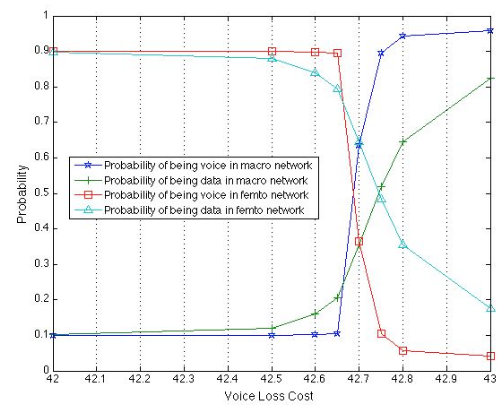
\includegraphics[height=3.9cm]{./Figures/lossProbabilities}
%      \caption {Comportamento de probabilidades \cite{green-markov}.}
			\label{figsnoop}}
		%\caption{Subfiguras}
		%\label{fig01}
	\end{figure}
  Quando o $\text{lossCost}_v = 42.7$, fluxo dividido (SCEN4).
\end{frame}

\begin{frame}
  \begin{block}{Recapitulando}
    \begin{itemize}
      \item SCEN1: Prioriza eficiência energética (intensidade de sinal)
      \item SCEN3: Prioriza QoS (vazão)
      \item SCEN4: Fluxo dividido
    \end{itemize}
  \end{block}
\end{frame}

\begin{frame}{Resultados}
  \begin{figure}[h]
  	\begin{center}
      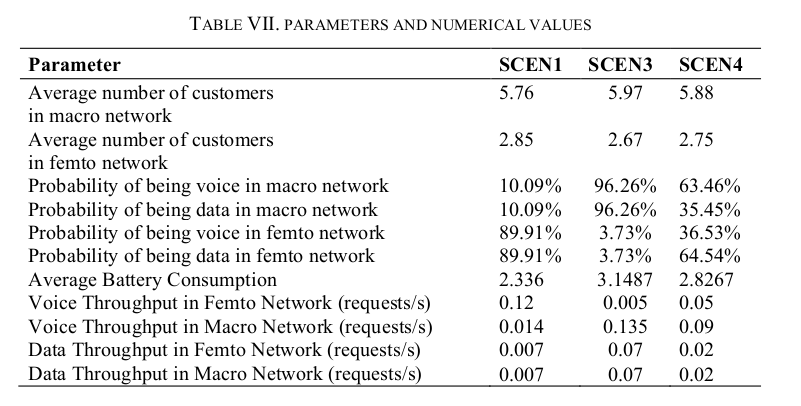
\includegraphics [scale=0.34]{./Figures/results}
     % \caption {Estimativa de dispositivos conectados à Internet.}
  		%\label{fig:arq-imuno}
  	\end{center}
  \end{figure}
  \begin{block}{Eficiência energética}
    \begin{itemize}
      \item SCEN4 aumenta $\approx 21\%$ em relação a SCEN1
      \item SCEN4 reduz em $\approx 10.22\%$ em relação a SCEN3
    \end{itemize}
  \end{block}
\end{frame}

\begin{frame}{Resultados}
  \begin{figure}[h]
  	\begin{center}
      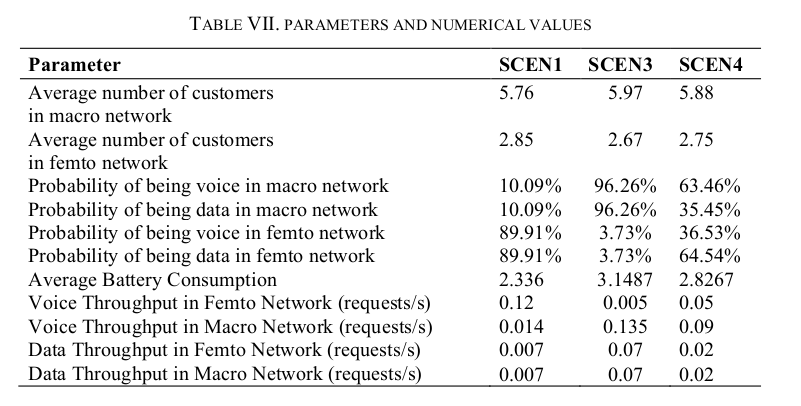
\includegraphics [scale=0.34]{./Figures/results}
     % \caption {Estimativa de dispositivos conectados à Internet.}
  		%\label{fig:arq-imuno}
  	\end{center}
  \end{figure}
  \begin{block}{Distribuição de carga - SCEN4 - Chamdas de Voz}
    \begin{itemize}
      \item \textit{macrocell}: $\approx 64\%$ ($loss = 0.5\%$, aceitável até
      $1\%$)
      \item \textit{femtocell}: $\approx 35\%$ ($loss = 2\%$)
    \end{itemize}
  \end{block}
\end{frame}

\begin{frame}{Resultados}
  \begin{figure}[h]
  	\begin{center}
      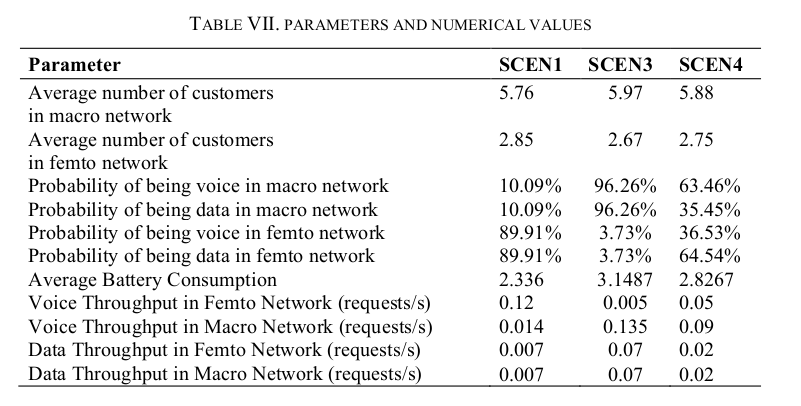
\includegraphics [scale=0.34]{./Figures/results}
     % \caption {Estimativa de dispositivos conectados à Internet.}
  		%\label{fig:arq-imuno}
  	\end{center}
  \end{figure}
  \begin{block}{Distribuição de carga - SCEN4 - Dados}
    \begin{itemize}
      \item Distribuição oposta
      \item Esperado pois a \textit{famtocell} tem melhor vazão
    \end{itemize}
  \end{block}
\end{frame}

\begin{frame}{Resultados}
  \begin{block}{}
    \begin{itemize}
      \item A política ótima proposta mantém alto nível de qualidade de
      serviço, enquanto minimiza o consumo de energia
      \item Balanceamento dos conceitos de \textit{Green Network} e
      \textit{Quality of Service}
    \end{itemize}
  \end{block}
\end{frame}

%\begin{frame}
%  \begin{block}{}
%    \begin{itemize}
%      \item
%    \end{itemize}
%  \end{block}
%\end{frame}

%\begin{frame}
%  \begin{block}{}
%  \end{block}
%\end{frame}

%\begin{frame}
%  \begin{figure}[h]
%  	\begin{center}
%      \includegraphics [scale=0.3]{./Figures/Device-Estimates}
%     % \caption {Estimativa de dispositivos conectados à Internet.}
%  		%\label{fig:arq-imuno}
%  	\end{center}
%  \end{figure}
%\end{frame}

%\begin{frame}{Redes de Acesso}
%	\begin{figure}[!htb]
%		\centering
%		\subfloat[DSL]{
%			\includegraphics[height=3.5cm]{./Figures/DSLaccess}
%			\label{figdroopy}}
%		\quad %espaco separador
%		\subfloat[Cable]{
%			\includegraphics[height=3.5cm]{./Figures/CableAccess}
%			\label{figsnoop}}
%		%\caption{Subfiguras}
%		%\label{fig01}
%	\end{figure}
%\end{frame}

%\begin{frame}[fragile]
%\scriptsize
%\begin{verbatim}
%\end{verbatim}
%\end{frame}
